% Ausgangslage (Ist-Analyse)

\section{Ausgangslage}
\label{sec:Ausgangslage}

\subsection{Anwendungsumfeld}
\label{subsec:Anwendungsumfeld}

%TODO
% Freistellen
\begin{wrapfigure}{l}{0.4\textwidth}
  \begin{center}
  	\vspace{-20pt}
	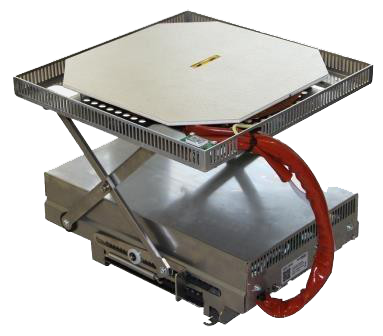
\includegraphics[scale=0.4]{analysis/res/einbaugeraete}
	\caption{Induktionsherd}
	\vspace{-40pt}
  \end{center}
\end{wrapfigure}

Die Firma Fluxron AG mit Sitz in Amriswil TG bietet induktive Heiz- und Energiesysteme für Grossküchen an. Die Produktpalette besteht aus verschiedenen Induktionsherden und Thermostatsystemen. Diese haben jeweils ein Bluetoothmodul eingebaut, welches auf ein CANopen-basiertes Protokoll zur Kommunikation setzt. Die Module liefern neben den Geräteeinstellungen auch Fehlercodes und Sensormesswerte via Blootooth.

Fluxron verkauft diese Induktionsgeräte an Servicefirmen, welche diese dann beim Endkunden, z.B. einem Restaurant, einbauen und installieren. Dabei, aber auch bei Wartungsarbeiten, setzen die Servicefirmen die bestehende Android Applikation \enquote{FLX Tool} zur Diagnose und zur Konfiguration ein.

Neben den Servicefirmen, setzen auch die Mitarbeiter der Firma Fluxron die Androidapplikation bei internen Versuchen oder zur Ferndiagnose ein. Bei der Ferndiagnose wird eine Teamviewer-Verbindung auf das Smartphone oder den PC des Technikers aufgebaut. Über diese kann dann eine Diagnose mittels den Tools via Bluetooth erfolgen.

\subsection{Bestehende Android-Applikation - FLX Tool }
\label{subsec:Bestehende Smartphone-Applikation}
In Eigenentwicklung wurde bei Fluxron bereits eine einfache Android-Applikation entwickelt. Diese unterstützt bereits das Suchen von Geräten, sowie das Lesen und Schreiben von Parametern. Da diese App allerdings immer nur ein Gerät gleichzeitig bedienen kann und die Benutzerinteraktion daher sehr Zeitaufwändig ist, soll im Rahmen dieses Projektes eine neue, übersichtlichere Androidapplikation entstehen. In den nachfolgenden Abschnitten sind die Funktionen dieser Applikation genauer aufgelistet.

\subsubsection{Suchlauf}
\label{subsubsec:Suchlauf}
Mit dem Suchlauf werden alle momentan aktiven Geräte gesucht und in einer Liste mit ihrer Device-ID aufgeführt. In der Liste sind neben den aktiven Geräten auch alle Geräte aufgelistet, welche schon einmal mit der App verbunden waren.

Nun kann man sich mit einem Gerät aus der Liste verbinden über in die Detailansichten mit dem Gerät zu interagieren.

\subsubsection{Ansichten je ein Kapitel pro view}
\label{subsubsec:Ansichten}
%TODO

\subsubsection{Einschränkungen der App}
\label{subsubsec:Einschränkungen der App}
\begin{itemize}
\item Es kann immer nur ein Gerät gleichzeitig verbunden sein
\item Für jede Verbindung ist ein erneuter Suchlauf nötig
\item Die Geräte sind nur mit der ID sichtbar, dies macht die Orientierung in einer Grossküche mit einem dutzend Geräten schwierig
\item Wenn ein nicht verbundenes Gerät eine Fehlermeldung absetzt, wird diese nicht empfangen
\end{itemize}

\subsection{Weitere bestehende Software}
\label{subsec:Weitere bestehende Software}
\subsubsection{FLX Access}
\label{subsubsec:FLX Access}
\begin{wrapfigure}{l}{0.5\textwidth}
  \begin{center}
  	\vspace{-26pt}
	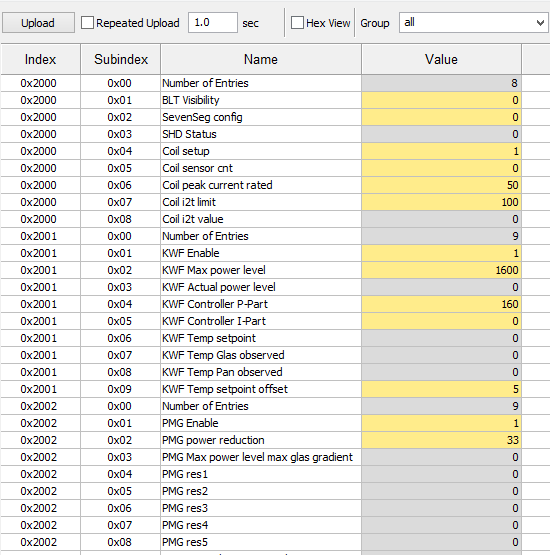
\includegraphics[scale=0.5]{analysis/res/flxaccess}
	\caption{FLX Access}
	\vspace{-140pt}
  \end{center}
\end{wrapfigure}

Mit FLX Access stellt Fluxron ein Windows-Tool zum auslesen und setzen von gerätespezifischen Parametern bereit. Die Kommunikation erfolgt via Bluetooth. Zudem kann der Gerätestatus ausgelesen werden. 

Dieses System ist besonders für die Entwicklungsphase von Geräten gedacht.%Wenn hier noch mehr Text kommt, dann vspace anpassen
\vspace{100pt}
\subsubsection{FLX Downloadtool}
\label{subsubsec:FLX Downloadtool}
\begin{wrapfigure}{l}{0.5\textwidth}
  \begin{center}
  	\vspace{-26pt}
	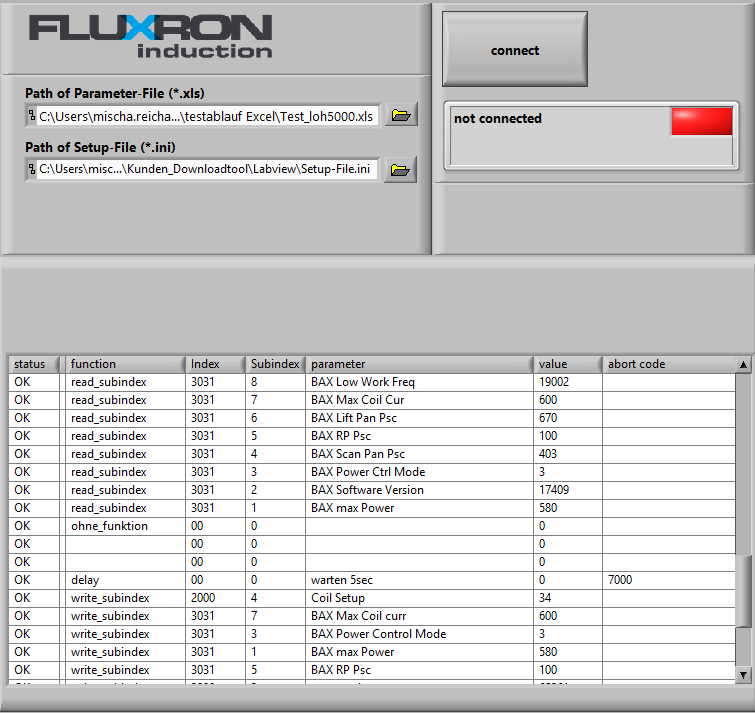
\includegraphics[scale=0.35]{analysis/res/flxdltool}
	\caption{FLX Downloadtool}
	\vspace{-100pt}
  \end{center}
\end{wrapfigure}

Das FLX Downloadtool ermöglicht den Download der gesamten Konfiguration in eine Excel-Datei. In dieser können dan die Parameter eingestellt werden. Danach werden die Einstellungen über das Tool wieder auf das Gerät geladen.

Eingesetzt wird dieses Programm für das Schreiben von kundenspezifischen Parametern auf mehrere Geräte.
%Wenn hier noch mehr Text kommt, dann vspace anpassen
\vspace{160pt}